% This is samplepaper.tex, a sample chapter demonstrating the
% LLNCS macro package for Springer Computer Science proceedings;
% Version 2.20 of 2017/10/04
%
\documentclass[runningheads]{llncs}
%
\usepackage{graphicx}
\usepackage{enumitem}
\usepackage{amsmath,amssymb}
\usepackage{mathtext}

\newcommand{\sign}{\operatorname{sign}}

%%%% ДЛЯ РУССКОГО ТЕКСТА закомментировать потом!
%\usepackage[utf8x]{inputenc}
%\usepackage[english,russian]{babel}
%\usepackage{cmap}
%%%%


% If you use the hyperref package, please uncomment the following line
% to display URLs in blue roman font according to Springer's eBook style:
% \renewcommand\UrlFont{\color{blue}\rmfamily}

\begin{document}
%
\title{An algorithm for searching the global minimum of univariate discontinuous functions\thanks{This work was supported by project no. 0729-2020-0055.}}
%
\titlerunning{An algorithm for searching the global minimum}
% If the paper title is too long for the running head, you can set 
% an abbreviated paper title here
%
\author{Konstantin Barkalov %\orcidID{0000-0001-5273-2471}  
\and Marina Usova %\orcidID{0000-0002-8736-0652}
}
%
\authorrunning{K. Barkalov, M. Usova}
% First names are abbreviated in the running head.
% If there are more than two authors, 'et al.' is used.
%
\institute{Lobachevsky State University of Nizhni Novgorod, Nizhni Novgorod, 
Russia \email{konstantin.barkalov@itmm.unn.ru}}
%
\maketitle              % typeset the header of the contribution
%
\begin{abstract}

\keywords{Global optimization \and Multiextremal functions \and 
Dimensionality reduction \and Peano curve \and Nested optimization \and 
Numerical methods.}

\end{abstract}
%
%
%
\section{Introduction}

$x^*$

$\varphi(x)$

\begin{equation}\label{problem}
\varphi(x^*)=\min\left\{\varphi(x):x\in\left[a,b\right]\right\}.
\end{equation}

(see, for example, popular approaches in \cite{Sergeyev2013}, \cite{PaulaviciusZilinskas2014}, \cite{Sergeyev2017}).

(\ref{problem})

\cite{Horst1995}, \cite{Horst1996}, \cite{Pinter1996})

$\varphi(x)$

$\varphi(x)$  $L$

\[
\left|\varphi(x')-\varphi(x'')\right|\leq L\left|x'-x''\right|,\; x',x'' \in [a,b].
\]

\cite{Jones2009}, \cite{Evtushenko2009}, \cite{Paulavicius2011}, \cite{Evtushenko2013}. 

\begin{itemize}
  \item
  \item 
  \item
\end{itemize}

\cite{Moreau2000}, \cite{Batukhtin1993}, \cite{Batukhtin1998}
\cite{Ban2019}, \cite{ZhangXu}

\cite{Strongin2000}

 MATLAB Global Optimization Toolbox \cite{MatlabOTB}. Section 6 concludes the paper. 


\section{2}

(\ref{problem})

objective function $\varphi(x):x\in[a,b]$

\begin{equation}\label{points}
a = \omega_0 <\omega_1 < ... <\omega_s < \omega_{s+1} = b.
\end{equation}


\begin{equation}\label{LipschitzСondition}
\left|\varphi(x')-\varphi(x'')\right|\leq L\left|x'-x''\right|,\; x',x'' \in (\omega_{i-1},\omega_{i}), 1 \leq i \leq s+1.
\end{equation}

$\omega_{0}$ and $\omega_{s+1}$

$\Omega$ $\Omega = \{\omega_{0}, ..., \omega_{s+1}\} \omega_{0} = a, \omega_{s+1} = b$

\cite{Strongin2000}

$s+1$

$x^i \in (\omega_{i-1},\omega_{i}), 1 \leq i \leq s+1 $

$x^{k+1}$, $k \geq s+1$

$x^1,…,x^k$

$\omega_{0}, ..., \omega_{s+1}$

$x_i, 0\leq i \leq m = k + s + 1$

\begin{equation}\label{pointsX}
a = x_0 < x_1 < ... < x_{m-1} < x_{m} = b,
\end{equation}

$z_i=\varphi(x_i)$

$x_i \not\in \Omega$

$(x_{i-1},x_i )$

$(x_{i-1},x_i ), 1\leq i \leq m$

\begin{equation}\label{mu_i}
\mu_i=(1-\gamma_i-\gamma_{i-1} )  \frac{|z_i-z_{i-1} |}{(x_i-x_{i-1} )}
\end{equation}

\begin{equation}\label{gamma}
\gamma_i = 
\begin{cases}
	1, &\text{$x_i \in \{\omega_{0},...,\omega_{s+1}\} $} \\
	0, &\text{$x_i \not\in \{\omega_{0},...,\omega_{s+1}\} $}
\end{cases}
\end{equation}


\begin{equation}\label{mu}
\mu=\max\left\{\mu_i: 1 \leq i \leq m\}\right\}
\end{equation}

$\mu=0$ $\mu=1$

$ 0 \leq \gamma_i+\gamma_{i-1} \leq 1$

$ 1 \leq i \leq m$

 $\mu_i$

 $0$

$ (x_{i-1},x_i ),1 \leq i \leq m$

$\Omega$

$(x_{i-1},x_i ), 1\leq i \leq m$

\begin{equation}\label{R_i}
R(i)=(1+\gamma_i+\gamma_{i-1} )\Delta_i+(1-\gamma_i-\gamma_{i-1} ) \frac{ (z_i-z_{i-1} )^2}{(r\mu)^2 \Delta_i }  -\frac{2[(1-\gamma_i )(1+\gamma_{i-1} ) z_i+(1+\gamma_i )(1-\gamma_{i-1} ) z_{i-1} ]}{r\mu}
\end{equation}

$r>1$

\begin{equation}\label{R}
R(t)=\max\left\{R(i): 1 \leq i \leq m\}\right\}
\end{equation}


\begin{equation}\label{new_x}
x^{k+1}=\frac {(x_t+x_{t-1})}{2}-(1-\gamma_t-\gamma_{t-1} ) \frac{(z_t-z_{t-1})}{2r\mu}
\end{equation}

$x_t-x_{t-1} \leq \epsilon$

$\epsilon > 0$


\begin{equation}\label{testFunction}
\varphi(x) =  0.1\sum_{i=1}^5{i\sin{(10(i+1)x+i)}}+
\begin{cases}
	-4, &0 \leq x < 3.1\\
	10, &3.1 \leq x < 4.6\\
	0, &4.6 \leq x < 7.0\\
	30, &7.0 \leq x < 9.0\\
	0, &9.0 \leq x \leq 10.0
\end{cases}
\end{equation}

$x\in[0,10]$ 

$r=2.0,\epsilon=0.001$

\begin{figure}[!ht]
	\begin{center}
			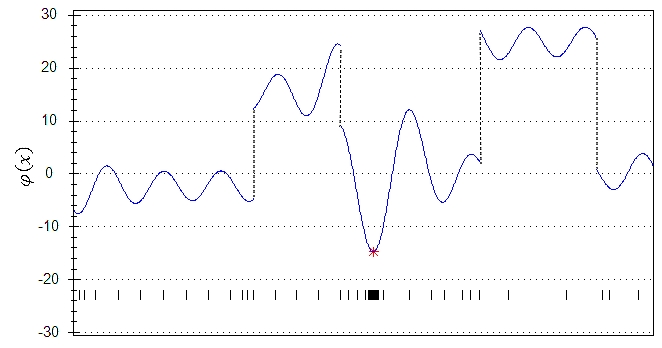
\includegraphics[width=0.9\linewidth]{ris_1.jpg}
			\caption{Fig.1}
      \label{ris1}
	\end{center}
\end{figure}

\section{3}

$\varphi(x)$

$\omega \in(x_{i-1},x_i)$

$\mu_i$

$\mu_i$

$(x_{i-1},x_i)$

$\mu_i$

\begin{equation}\label{mu_cond}
\mu(1) \leq \mu(2) \leq ... \leq \mu(m)
\end{equation}

\begin{equation}\label{mu_main_cond}
 \frac{\mu(p)}{\mu(p+1)} \leq Q, 1 \leq p < q(m-2(s+1))
\end{equation}

$Q >1$ and $0<q<1$

$\mu_i$

$p<m-2(s+1)$

$1 \leq p<q(m-2(s+1))$

$\mu_i$

$I=\{i:1 \leq i \leq m,\mu_i=\mu(j),1 \leq j \leq p\}$

$(x_{i-1},x_i)$

$\mu_i$

$(x_{i-1},x_i), i \in I$

\section{4}

$x^i \in (\omega_{i-1},\omega_i ),1 \leq i \leq s+1$

$\Omega=\{\omega_0,…,\omega_{s+1}\}$

$\omega_0=a$ and $\omega_{s+1}=b$

$x^{k+1}, k \geq s+1$

$\{x^1,...,x^k\} \cup \Omega$

\begin{equation}\label{x_cond}
 a=x_0<x_1<...<x_{m-1}<x_m=b,
\end{equation}

$m=s+k+1$

$\gamma_i$

$z_i=\varphi(x_i )$

$ x_i \not\in \Omega$

$\gamma_i=0$

$\mu_i,1 \leq i \leq m$

$0<q<1<Q$

\begin{equation}\label{delta_cond}
\delta_i=
\begin{cases}
	\sign{(z_i - z_{i-1})}, &\text{$i \in I$} \\
	0, &\text{$i \not \in I$}
\end{cases}
\end{equation}

$\delta_i=-1$

$(x_{i-1},x_i ), \delta_i=1$

$\delta_i=0$

$ 0 \leq \gamma_i+\gamma_{i-1}+|\delta_i | \leq 1$

$1 \leq i \leq m$

\begin{equation}\label{mu_new}
\mu=\max\left\{(1-\gamma_i-\gamma_{i-1}-|\delta_i|) \frac {|z_i-z_{i-1}|}{(x_i-x_{i-1})}: 1 \leq i \leq m\}\right\}
\end{equation}

$\mu=0$ $\mu=1$

$(x_{i-1},x_i), 1 \leq i \leq m$

\begin{equation}\label{mu_new}
\begin{gathered}
R(i)=(1+\gamma_i+\gamma_(i-1)+|\delta_i |) \Delta_i+(1-\gamma_i-\gamma_{i-1}-|\delta_i |)\frac{(z_i-z_{i-1} )^2}{(r\mu)^2 \Delta_i } \\
- \frac{2[((1-\gamma_i )(1+\gamma_{i-1} )(1-\delta_i )) z_i+((1+\gamma_i )(1-\gamma_{i-1} )(1+\delta_i )) z_{i-1} ]}{r\mu}
\end{gathered}
\end{equation}

$\mu$ $\Delta_i=x_i-x_{i-1}$

\begin{equation}\label{R}
R(t)=\max\left\{R(i): 1 \leq i \leq m\}\right\}
\end{equation}

\begin{equation}\label{new_x_2}
x^{k+1}=\frac {(x_t+x_{t-1})}{2}-(1-\gamma_t-\gamma_{t-1}- |\delta_t|) \frac{(z_t-z_{t-1})}{2r\mu}
\end{equation}

$x_t-x_{t-1} \leq \epsilon$

$\epsilon > 0$

$r=2.0,\epsilon=0.001,Q=3.0,q=0.3$

\begin{figure}[!ht]
	\begin{center}
			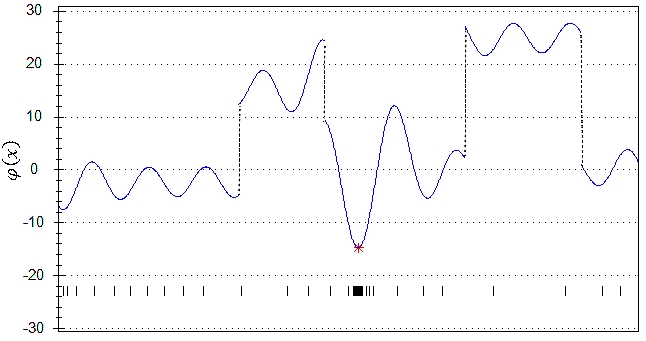
\includegraphics[width=0.9\linewidth]{ris_2.jpg}
			\caption{Fig.2}
      \label{ris2}
	\end{center}
\end{figure}

\begin{figure}[!ht]
	\begin{center}
			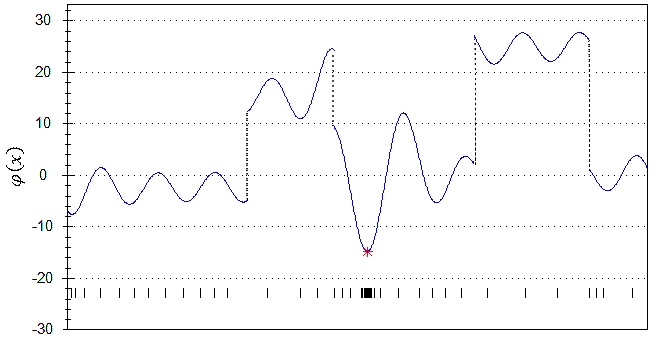
\includegraphics[width=0.9\linewidth]{ris_3.jpg}
			\caption{Fig.3}
      \label{ris3}
	\end{center}
\end{figure}

$r=2.0,\epsilon=0.001,Q=3.0,q=0.3$

\section{Results of Numerical Experiments}

\cite{Audet}
\cite{Goldberg}
\cite{Kirkpatrick}
\cite{MatlabOTB}

\begin{equation}\label{seriaFunction}
f(x) =  \sum_{i=0}^4{(j+1)A_j\sin{(5\pi jx+j)}+(j+1)B_j\cos(3\pi jx+j)}, x\in[0,1]
\end{equation}

$A_j,B_j$

$[-6,6]$

$\omega_1,\omega_2,\omega_3,\omega_4$

$[0,0.25), [0.25,0.5), [0.5,0.75), [0.75,1]$

$\delta_1,\delta_2,\delta_3,\delta_4$

$[-50,50]$

\begin{equation}\label{seriaFunction_jump}
\varphi(x) =  f(x)+
\begin{cases}
	\delta_1, &0 \leq x < \omega_1\\
	\delta_2, &\omega_1 \leq x < \omega_2\\
	\delta_3, &\omega_2 \leq x < \omega_3\\
	\delta_4, &\omega_3 \leq x < \omega_4\\
	\delta_1, &\omega_4 \leq x \leq 1.0
\end{cases}
\end{equation}

$x\in[0,1]$

global optimizer $x^*$

$x^k$

$|x^k-x^* | \leq \delta$

$x^*$

$\delta= 10^{-2}$

$\epsilon = 10^{-3}$

$x_0$

 MATLAB Global Optimization Toolbox

$r=2.2$

\begin{table}[h]
	\caption{Results}
	\begin{center}
		\begin{tabular}{|c|c|c|c|}
			\hline
			Method & Solved & Sr count of iteration & Sr funccount \\
			\hline
			\hline
                                AGS-D & 1000  &  52  &  53 \\
                                \hline
                                SA    &  1000  &  774  &  777  \\
			\hline
			GA    &   999  &  24  &  1290  \\
			\hline
                                DS    &  970  & 38  &  71  \\
			\hline
		\end{tabular}
	\end{center}
\end{table}

$r=3.7,Q=3.0,q=0.3$

\begin{table}[h]
	\caption{Results 2}
	\begin{center}
		\begin{tabular}{|c|c|c|c|}
			\hline
			Method & Solved & Sr count of iteration & Sr funccount \\
			\hline
			\hline
                                AGS-D & 1000  & 79  &  80 \\
                                \hline
                                SA    &  998  &  765  &  770  \\
			\hline
			GA    &   993  &  25  &  1310  \\
			\hline
                                DS    &  964  & 38  &  71  \\
			\hline
		\end{tabular}
	\end{center}
\end{table}




Word order:

\cite{Sergeyev2013}
\cite{PaulaviciusZilinskas2014}
\cite{Sergeyev2017}
\cite{Horst1995}
\cite{Horst1996}
\cite{Pinter1996}
\cite{Jones2009}

\cite{Evtushenko2009}
\cite{Paulavicius2011}
\cite{Evtushenko2013}
\cite{Strongin2000}

\cite{Moreau2000}

\cite{Batukhtin1993}
\cite{Batukhtin1998}
\cite{Ban2019}

\cite{ZhangXu}
\cite{Audet}

\cite{Goldberg}
\cite{Kirkpatrick}
\cite{MatlabOTB}


\section{Conclusion}




%
% ---- Bibliography ----
%
% BibTeX users should specify bibliography style 'splncs04'.
% References will then be sorted and formatted in the correct style.
%
 \bibliographystyle{splncs04}
 \bibliography{bibliography}


\end{document}
